\section{Background estimation}
\label{sec:dihiggs_backgrounds}

%-------------------------------------------------------------------------------
In the present analysis we expect that at the end of the selection the
sample will be largely dominated by $t \bar{t}$ background, therefore the $t\bar{t}$ background normalisation
is derived from data. As described in Sec. \ref{sec:multijet}, the multi-jet
background is derived using the data-driven matrix method.
For all other backgrounds, e.g. di-boson, Higgs, $W$+jets, the
MC is used appropriately normalised using the expected cross sections and the
integrated luminosity that has been collected.

\subsection{Top normalisation and control region}
\label{subsec:topCR}
The top background is the major background source in this analysis,
therefore dedicated control regions (CR) are used to check its modeling
and to normalise it. Two CR's are defined, one for the SR's optimised for
the $m_h = 700$ GeV signal hypothesis (low mass analysis
in the following) and the other for the $m_h = 2000$ GeV signal (high mass
analysis in the following). The two CRs are defined in Table \ref{tab:CRdef}.

\begin{table}
\caption{Definition of the kinematic regions used to normalise the Top background.} \label{tab:CRdef}
\begin{center}
\begin{tabular}{c|c}
\hline
\multicolumn{2}{c}{Top CR definitions} \\
\hline
low mass &  ($m_{bb} < 100$ GeV or $m_{bb} > 140$ GeV ) and $p_T^{\rm bb} > 150$ GeV \\
high mass &   ({$m_{bb} < 100$ GeV or $m_{bb} > 140$}) and $p_T^{\rm bb} > 350$ GeV \\
\hline
\end{tabular}
\end{center}
\end{table}


Table \ref{tab:CR1} and \ref{tab:CR2} show the number of observed
events and expected background events in the top CR. 

\begin{table}
\caption{Data and expected background yields in the low mass control
  region. NF of 1.12 has been applied to $t\bar{t}$ background.} \label{tab:CR1}
 \begin{center}
 \begin{tabular}{c | c c c|} 
 \hline
   Sample       &  Yields      & error      \\
   \hline
   \hline
        Signal(750)        &   11.4  &     0.3   \\
        \hline
         $t\bar{t}$        &  68623.2      & 137.37   \\%tt normalized to Data

        \hline
             $W$+jets        &   7917.67      & 204.31     \\

          \hline
       Single Top  & 7064.57       & 36.03\\  
       %$W\to \tau \nu+b$-jet         &  55.43   &    6.65    \\
      %$W\to \mu \nu+b$-jet         &  455.25    &   58.55    \\
      %$W \to e \nu+b$-jet         &   494.99    &   113.67   \\
      %$W \to \tau \nu+c$-jet       &    45.84     &    10.40  \\
      %$W \to  \mu \nu+c$-jet      &      227.29       &10.36    \\ 
      %$W \to e \nu+c$-jet      &      450.89  &     14.73     \\
      %$W \to \tau \nu+$light-jet        &   14.95   &    8.87     \\
      %$W \to \mu \nu+$light-jet         & 89.34    &   12.27     \\
      %$W \to e \nu+$light-jet    & 66.54    &   12.27    \\
        \hline
             $Z$+jets        &   2159.88      & 132.05     \\
             
         \hline
         QCD        & 2041.52        & 72.19\\

         \hline 
        Dibosons & 850.15     & 20.12\\
        \hline
        \hline

              tot bkg. & 88799.2 & 288.77 \\
        \hline
             data & 88799 & \\
        \hline
\end{tabular}
\end{center}

\end{table}

\begin{table}
\caption{Data and expected background yields in the high mass control
  region. NF of 1.05 has been applied to $t\bar{t}$ background.} \label{tab:CR2}
 \begin{center}
 \begin{tabular}{c | c c c c|} 
 \hline
    Sample         & Yield         & error \\
\hline
\hline
       Signal(2000)  &     3.80 &     0.16     \\
       
\hline
         $t\bar t$           & 2957.63    &   28.04    \\
\hline

       $W$+jets          & 693.18    &   28.30      \\       
       
      %$W\to \tau \nu+b$-jet     &    4.54  &    0.81      \\
       %$W\to \mu \nu+b$-jet    &   87.57   &    26.14      \\
       %$W\to e \nu+b$-jet      &  37.65    &   2.28     \\
      %$W\to \tau \nu+c$-jet      & 3.44     &  1.09      \\
       %$W\to \mu \nu+c$-jet     & 19.12     &  1.63      \\
       %$W\to e \nu+c$-jet      &     37.46   &    2.72      \\
       %$W\to \tau \nu+$-light jet    &   0.48    &   0.19      \\
       %$W\to \mu \nu+$-light jet       &   6.36     &  1.96      \\
       %$W\to e \nu+$-light jet         &  4.84   &   0.68      \\
\hline
        $Z$+jets          & 156.12    &   9.49      \\
\hline
        Single Top  & 726.33       & 11.55\\  
 \hline
        Dibosons  & 133.88      & 7.31\\  
 \hline
        QCD & 161.34      &18.2\\
 
  
\hline
\hline
     tot bkg. & 4841. & 42.87 \\
     \hline
    data & 4848 & \\
\hline
\end{tabular}
\end{center}

\end{table}


The top normalisation factors are determined by a simultaneous fit  of
signal and control regions. It also depends slightly on the $m_{hh}$ window due to the presence of top background in the signal region, and it is furthermore different for the \emph{low  mass} and \emph{high mass} analyses. The normalisation
factors of the two top control regions are shown in Table \ref{tab:NFs}.
\begin{table}
\caption{Normalisation factors for the two CRs, the statistical error
  includes only data statistics, the systematic error is shown to
  check the compatibility of the NF with one, but it is not directly
  used in the fit procedure.} \label{tab:NFs}
\begin{center}
\begin{tabular}{c|c|c|c}
\multicolumn{4}{c}{Top background normalisation factors in the two
  CRs} \\
\hline
region & NF & $\sigma_{stat.}$ & $\sigma_{syst.}$ \\
\hline
low mass & 1.12 & 0.005 & 0.21 \\
high mass & 1.05 & 0.03 & 0.36 \\
\hline
\end{tabular}
\end{center}
\end{table}

Table \ref{tab:CR1} and \ref{tab:CR2} show the number of observed
events and expected background events in the top CR after the
normalisation factors have been applied to the top background sample.

Fig.~\ref{fig:mbb_mhh} shows the $m_{bb}$ and $m_{hh}$ distributions in the two CRs while n Appendix \ref{app:CR1} and \ref{app:CR2} we show the complete distributions of the
relevant variables used in the analysis selection in the top CR.  

\begin{figure}[!h]
\begin{center}
\includegraphics*[width=0.47\textwidth] {chapters/dihiggs/figures/ControlPlots/CR1/C_mBBcr_opt700_bbpt150_bbMass.eps}
\includegraphics*[width=0.47\textwidth] {chapters/dihiggs/figures/ControlPlots/CR1/C_mBBcr_opt700_bbpt150_hhMass.eps}
\includegraphics*[width=0.47\textwidth] {chapters/dihiggs/figures/ControlPlots/CR2/C_mBBcr_opt2000_bbpt350_bbMass.eps}
\includegraphics*[width=0.47\textwidth] {chapters/dihiggs/figures/ControlPlots/CR2/C_mBBcr_opt2000_bbpt350_hhMass.eps}
\caption[$m_{bb}$ and $m_{hh}$ in CR1 and CR2.]{$m_{bb}$ and $m_{hh}$ in CR1 and CR2.  }
\label{fig:mbb_mhh}
\end{center}
\end{figure}
%%%%%%%
\clearpage

\subsection{Multi-jet background}
\subsection{Multi-jet background}
\label{sec:multijet}
Multi-jet backgrounds can enter in the event selection if a jet from
heavy flavour decays is mis-identified as an electron or a muon and used
as a lepton in the analysis. Such phenomena are not reproduced by MC
simulation, due to large uncertainties in the jet shower shape simulation
and uncertainties in muon fragmentation functions and kinematics. Therefore
a data driven method based on the Matrix Method estimation technique
described in detail in Ref.~\cite{ConfMM} is used to estimate this
background in the present analysis.
%%Such methods are used extensively in the top group analyses.

The method is based on the use of two lepton types, loose leptons and
tight leptons. The tight leptons are those used in the signal analysis,
while loose leptons are used for the multi-jet background estimation. Note that the tight leptons are a subset of the loose leptons. The
idea of the method is to estimate the number of ``fake'' leptons passing
the tight lepton requirements by computing:

\begin{enumerate}
\item the number of loose leptons;
\item the number of tight leptons;
\item the probability that a fake lepton is reconstructed as a tight
      lepton ($\epsilon_{\rm fake}$);
\item the probability that a real lepton is reconstructed as a tight
      lepton ($\epsilon_{\rm real}$)
\end{enumerate}

Such quantities enter in the Matrix Method through the following expressions:
\begin{eqnarray*}
N_{\rm loose} & = & N^{\rm real}_{\rm loose} + N^{\rm fake}_{\rm loose} \\
N_{\rm tight} & = & \epsilon_{\rm real}N^{\rm real}_{\rm loose} + \epsilon_{\rm fake} N^{\rm fake}_{\rm loose}
\end{eqnarray*}
Solving the equation above,  the number of fake leptons passing the ``tight''
identification requirement is given by:
\[
N_{\rm fake}^{\rm tight} = \epsilon_{\rm fake}N^{\rm loose}_{\rm fake} = \frac{\epsilon_{\rm fake}}{\epsilon_{\rm real} - \epsilon_{\rm fake}} \left (\epsilon_{\rm real}N^{\rm loose} - N^{\rm tight} \right)
\]
The number $N_{\rm fake}^{\rm tight}$ is actually determined by running on a
``loose'' lepton data sample and weighting the events by the factor:
\[
w_i = \frac{\epsilon_{\rm fake}}{\epsilon_{\rm real} - \epsilon_{\rm fake}} \left (\epsilon_{\rm real} - 
\delta_i \right)
\]
where $\delta_{i}$ is one if the lepton is tight and zero otherwise.
The multi-jet background estimation is
validated using the observed $m_{\rm T}$ distribution in events in the
top control region with one $b$-tag, as shown in
Figure~\ref{fig:mwt}.
\begin{figure}
\begin{center}
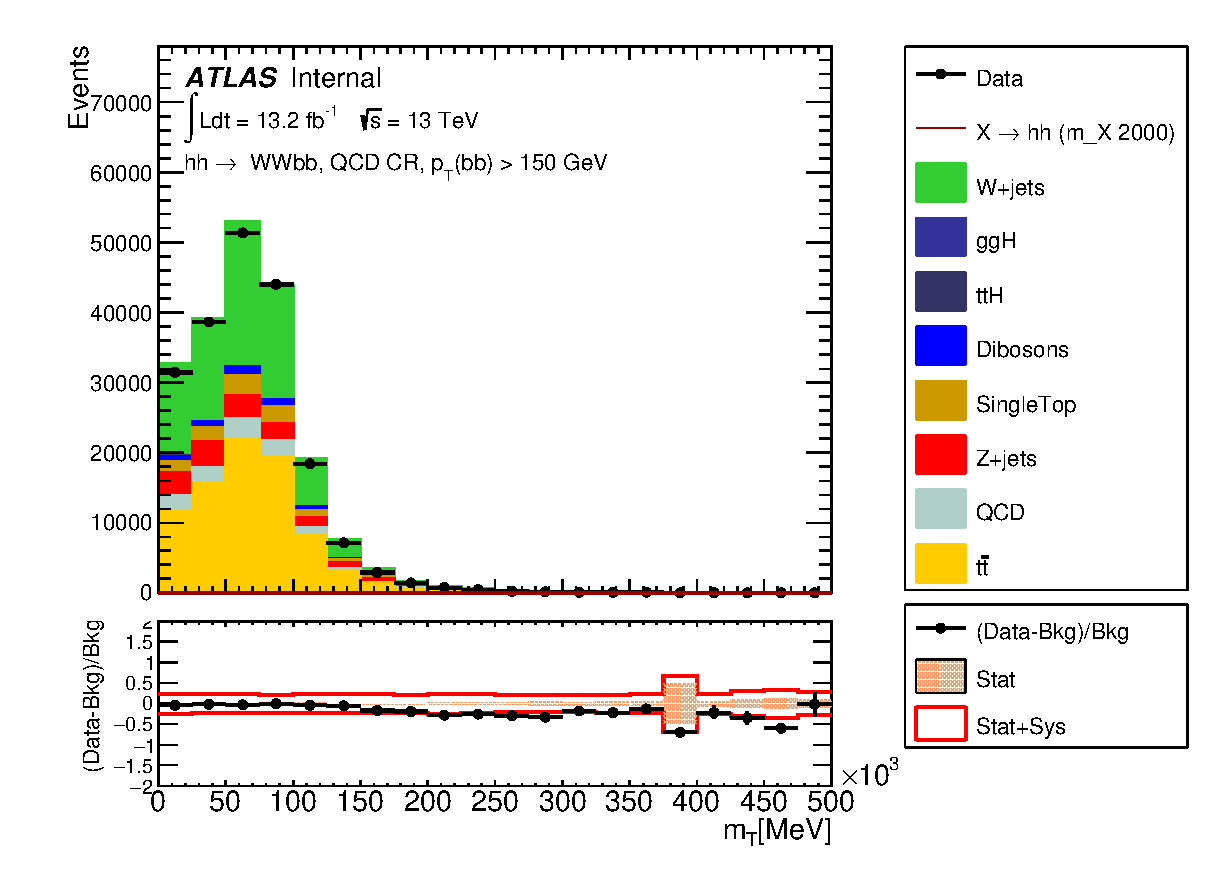
\includegraphics[width=0.47\textwidth, height=0.35\textwidth]{chapters/dihiggs/figures/C_bj1_opt700_bbpt150_wlepmtben.eps}
\includegraphics[width=0.47\textwidth, height=0.35\textwidth]{chapters/dihiggs/figures/ControlPlots/CR1/C_opt700_bbpt150_wlepmtben.eps}
\end{center}
\caption{$m_{\rm T}$ distribution for events in the QCD enriched control region
   with one $b$-tag (left) and with $t\bar{t}$ control region two $b$-tag (right).}
\label{fig:mwt}
\end{figure}










\clearpage


